\documentclass{abrice}

\title{Comp 549: Assignment 1}
\author{Anthony Brice}

\begin{document}
\maketitle

\section{Part 1}

\emph{Write a few observations about each of the given articles.}

\subsection{As we may think, Bush V.}

It surprises me that even by 1945 it was not taken for granted that information
would be digitized. Bush spends considerable length coming up with plausible
scenarios by which analog information can be encoded and decoded to facilitate
some of his ideas on distribution. Now we have digital information compressed to
far greater degrees than Bush envisioned that can be decoded by any other Turing
machine, no special equipment necessary.

While very prescient, his memex prediction gets one other crucial component of
the coming information explosion wrong. Bush posits that information stores will
be centralized and personal rather than distributed. He predicts hyper-linking
with astonishing clarity but fails to see how much more utility a society gleans
when the links point to content shared among everyone.

One last note: When Bush assigns a gender, he really means it. Jobs involving
rote mechanical work or pure data entry he invariably describes as
feminine. ``Girls'' are ``typists'' and ``stenographers,'' ``armed with simple
keyboard punches.'' To stark contrast, Bush describes his
``scientist''---someone ``who manipulates data and examines the world about him
by the use of logical processes''---invariably as masculine.


\subsection{Design-oriented human--computer interaction, Fallman D.}
\marginnote{Throughout his paper Fallman is compelled to join \textit{human} and
  \textit{computer} with an em dash. We do not reproduce here that typographical
  atrocity.}

\indent
Twelve years on, I don't think many would argue Fallman the points he makes
here. Many of the field's great success stories of the past decade have been due
in large part to making design a primary concern. Consider Apple, where
anonymous employees liken the design department to a holy priesthood, or Valve
Software, whose iterative design process changed the shape and course of the
multi-billion dollar games industry. Fallman goes on to show how an iterative
process naturally leads to his thesis that design should be considered more ``a
dialogue'' than a ``structured and linear process,'' and that is certainly a
claim Valve's process satisfies.

\section{Part 2}

\emph{Create a prototype of an interactive system for the following scenario:}

\emph{An insurance company would like to send field agents out to homes that
  have been damaged by wildfires and other natural disasters. They would like
  the agents to use a mobile device, such as a tablet, to photograph the damaged
  parts of the house so that they can be uploaded to an appraiser that can
  quickly calculate the settlement. The agent should be able to quickly enter
  the location of the home which should then show up on a map. The appraiser in
  the office should see the same interface as the agent and should be able to
  quickly view all of the photos, the location information, the names and
  account numbers if available and any notes that the agent has written.}

\bigskip

\begin{figure}
  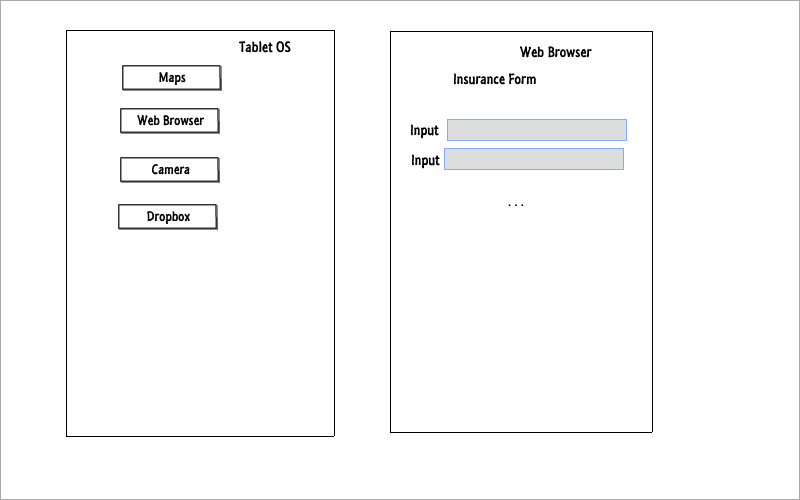
\includegraphics{foobar.jpg}
  \caption{Two screens from the interactive system.}
\end{figure}

\noindent
My prototype is nothing more than a traditional tablet with the assumption that
company has a web interface available through which the agent and appraiser can
share textual information about the current home. The prompt tries to lead us to
the conclusion that the company needs one application to handle mapping,
photography, and data entry, but as my prototype shows that is wholly
unnecessary. In fact, this ``build the app for that'' mentality is exactly the
kind railed against in Kernighan and Pike's \textit{Program Design in the Unix
  Environment}. (Insurance companies need their own maps app no more than UCB
needed its own implementation of \texttt{ls}.)

The only portion for which the company needs a custom application is for the web
forms. They'll need a server to serve up forms to the agent and to serve a page
to the appraiser to view the data input by the agent. The agent could also
upload photo files through this web form, but it might be easier to use a
utility specifically designed to facilitate sharing large files,
e.g.~Dropbox. Again, there's no reason why an insurance company needs their own
custom implementation of such a software utility.

\end{document}
%%% Local Variables:
%%% mode: latex
%%% TeX-master: t
%%% End:
